\documentclass{article} % For LaTeX2e
\usepackage[backend=bibtex, sorting=none]{biblatex}
\addbibresource{bibliography.bib}
\usepackage{graphicx}
\graphicspath{{figures/}}
\usepackage{nips15submit_e,times}
\usepackage{hyperref}
\usepackage{url}
\usepackage{amsmath}
\usepackage{tipa}
\usepackage{multicol}
\usepackage{multirow}
\usepackage[linesnumberedhidden,ruled,noend]{algorithm2e}
\usepackage{listings}
\usepackage{color}

\definecolor{dkgreen}{rgb}{0,0.6,0}
\definecolor{gray}{rgb}{0.5,0.5,0.5}
\definecolor{mauve}{rgb}{0.58,0,0.82}

\lstset{frame=tb,
  language=Python,
  aboveskip=3mm,
  belowskip=3mm,
  showstringspaces=false,
  columns=flexible,
  basicstyle={\small\ttfamily},
  numbers=none,
  numberstyle=\tiny\color{gray},
  keywordstyle=\color{blue},
  commentstyle=\color{dkgreen},
  stringstyle=\color{mauve},
  breaklines=true,
  breakatwhitespace=true,
  tabsize=3
}

\makeatletter
\def\BState{\State\hskip-\ALG@thistlm}
\makeatother
%\documentstyle[nips14submit_09,times,art10]{article} % For LaTeX 2.09

\title{COMPGW02: Web Economics\\Assignment 1 - Part B}

\author{
Sergiu Tripon\\
Department of Computer Science\\
University College London\\
Gower Street, London, WC1E\\
\texttt{sergiu.tripon.15@ucl.ac.uk}\\
}

% The \author macro works with any number of authors. There are two commands
% used to separate the names and addresses of multiple authors: \And and \AND.
%
% Using \And between authors leaves it to \LaTeX{} to determine where to break
% the lines. Using \AND forces a linebreak at that point. So, if \LaTeX{}
% puts 3 of 4 authors names on the first line, and the last on the second
% line, try using \AND instead of \And before the third author name.

\newcommand{\fix}{\marginpar{FIX}}
\newcommand{\new}{\marginpar{NEW}}

\nipsfinalcopy % Uncomment for camera-ready version

\begin{document}

\maketitle

\section{Convergence Criterion}

The convergence criterion employed throughout this assignment came in the form of a threshold. In order to establish an optimal threshold, the gradient descent was first run without a stopping condition. Mostly, the mean squared error decreased by larger portions at the very beginning of a test and then continued with a uniform, regular and slower decrease. This indicated that the curve was drawn and the gradient descent was now following a straight line (see red line on Figure \ref{Fig1}), which means convergence was achieved. The threshold was chosen based on error values post-convergence and epochs.

During each epoch, the mean squared error was compared with the set threshold, and if the error was smaller than the threshold, the test would stop. The threshold value varied from Linear Regression to Logistic Regression and from Stochastic Gradient Descent to Batch Gradient Descent. However, the "Last Epoch MSE" values provide an indication on the range of the threshold set.

For the purpose of the report, another stopping condition of a maximum of 500 epochs for SGD and 50 epochs for BGD was also introduced. 

\section{Linear Regression with Stochastic Gradient Descent \cite{ng2000cs229} \cite{roc_curve}}

\subsection{Training}

Table \ref{Table1} shows the mean squared error (MSE) on the last epoch when training Linear Regression with SGD for 500 epochs with 4 different learning rates. It was found that it produced the lowest MSE with a learning rate of 0.001.

Figure \ref{Fig1} provides a visual representation of the performance of Linear Regression with SGD trained with 4 different learning rates for 500 epochs.

\begin{table}[!htbp]
\caption{Linear Regression with SGD training with 4 different learning rates. Lowest MSE on the last epoch shown in \textbf{bold}.}
\label{Table1}
\begin{center}
\begin{tabular}{l l l l l}
\multicolumn{1}{c}{\bf Epochs} &\multicolumn{1}{c}{\bf Regression}  &\multicolumn{1}{c}{\bf Gradient Descent} &\multicolumn{1}{c}{\bf Learning Rate} &\multicolumn{1}{c}{\bf Last Epoch MSE}
\\ \hline \\

500 & Linear & Stochastic & 0.00001 & 0.19106040630421942\\
500 & Linear & Stochastic & 0.0001  & 0.17909130473210128\\

\textbf{500} & \textbf{Linear} & \textbf{Stochastic} & \textbf{0.001} & \textbf{0.17462479941829512}\\

500 & Linear & Stochastic & 0.01    & 0.18145635103672708\\

\end{tabular}
\end{center}
\end{table}

\clearpage

\begin{figure}[!htbp]
\begin{center}
\fbox{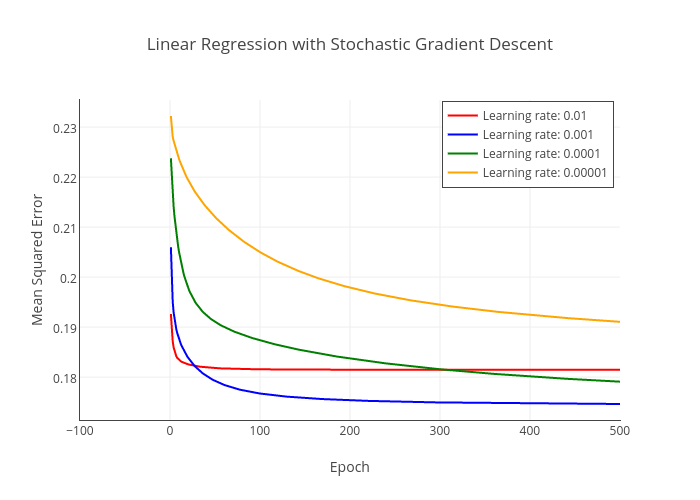
\includegraphics[width=12cm]{lin_sgd/lin_sgd_all}}
\end{center}
\caption{Linear Regression with SGD training with 4 different learning rates.}
\label{Fig1}
\end{figure}

\subsection{Evaluation}

\textbf{Receiver operating characteristic (ROC) Curve}

Figure \ref{Fig2} shows the ROC curve of Linear Regression with SGD trained with 4 different learning rates for 500 epochs.

Figure \ref{Fig3} shows the ROC curve of Linear Regression with SGD trained with the optimal learning rate identified for 500 epochs.

\begin{figure}[!htbp]
\begin{center}
\fbox{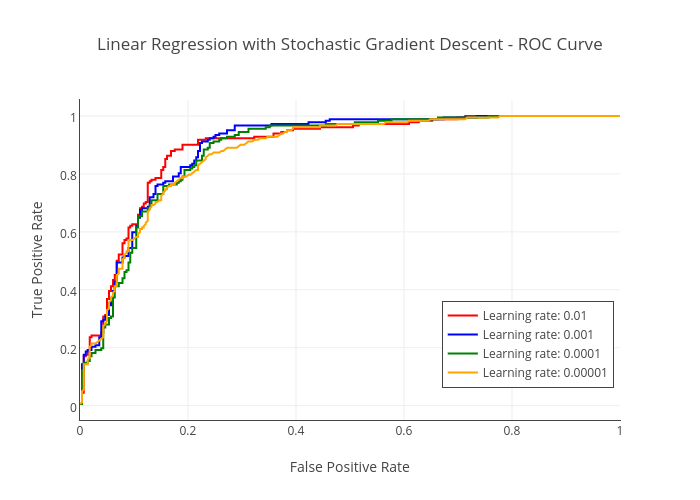
\includegraphics[width=12cm]{lin_sgd/lin_sgd_all_roc}}
\end{center}
\caption{ROC Curve of Linear Regression with SGD training with 4 different learning rates.}
\label{Fig2}
\end{figure}

\begin{figure}[!htbp]
\begin{center}
\fbox{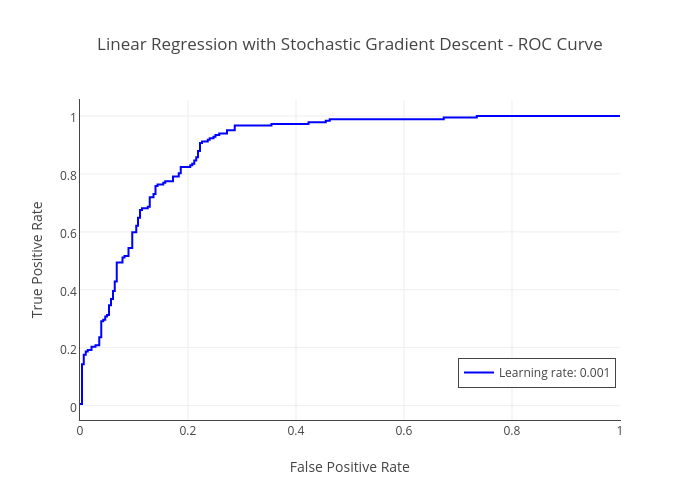
\includegraphics[width=12cm]{lin_sgd/lin_sgd_all_roc1}}
\end{center}
\caption{ROC Curve of Linear Regression with SGD training with optimal learning rate identified.}
\label{Fig3}
\end{figure}

\textbf{Area under the curve (AUC)}

Table \ref{Table2} shows the AUC (Area under the curve) of Linear Regression with SGD trained with 4 different learning rates for 500 epochs.

\begin{table}[ht]
\caption{AUC of Linear Regression with SGD trained with 4 different learning rates. Highest AUC shown in \textbf{bold}.}
\label{Table2}
\begin{center}
\begin{tabular}{l l l}
\multicolumn{1}{c}{\bf Epochs} &\multicolumn{1}{c}{\bf Learning Rate} &\multicolumn{1}{c}{\bf AUC}
\\ \hline \\

500 & 0.00001 & 0.8475914766237341\\
500 & 0.0001  & 0.8810311552247047\\

\textbf{500} & \textbf{0.001} & \textbf{0.8923549568710862}\\

500 & 0.01    & 0.8922958761668431\\

\end{tabular}
\end{center}
\end{table}

\clearpage

\section{Linear Regression with Batch Gradient Descent \cite{ng2000cs229} \cite{roc_curve}}

\subsection{Training}

Table \ref{Table3} shows the mean squared error (MSE) on the last epoch when training Linear Regression with BGD for 50 epochs with 6 different learning rates. It was found that it produced the lowest MSE with a learning rate of 0.000001.

Figure \ref{Fig4} provides a visual representation of the performance of Linear Regression with BGD trained on 2 different learning rates for 50 epochs.

\begin{table}[!htbp]
\caption{Linear Regression with BGD training with 6 different learning rates. Lowest MSE on the last epoch shown in \textbf{bold}.}
\label{Table3}
\begin{center}
\begin{tabular}{l l l l l}
\multicolumn{1}{c}{\bf Epochs} &\multicolumn{1}{c}{\bf Regression}  &\multicolumn{1}{c}{\bf Gradient Descent} &\multicolumn{1}{c}{\bf Learning Rate} &\multicolumn{1}{c}{\bf Last Epoch MSE}
\\ \hline \\

50 & Linear & Batch & 0.0000001 & 0.2494526190216533\\

\textbf{50} & \textbf{Linear} & \textbf{Batch} & \textbf{0.000001} & \textbf{0.22658756874338298}\\

50 & Linear & Batch & 0.00001   & diverged\\
50 & Linear & Batch & 0.0001    & diverged\\
50 & Linear & Batch & 0.001     & diverged\\
50 & Linear & Batch & 0.01      & diverged\\
\end{tabular}
\end{center}
\end{table}

\begin{figure}[!htbp]
\begin{center}
\fbox{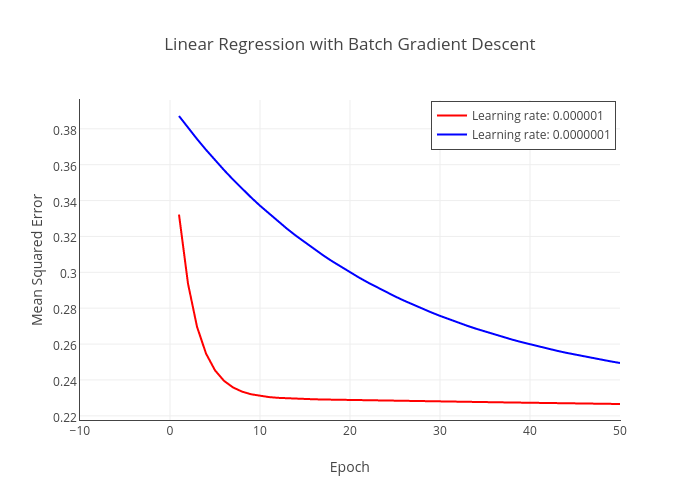
\includegraphics[width=12cm]{lin_bgd/lin_bgd_all}}
\end{center}
\caption{Linear Regression with BGD training with 2 different learning rates.}
\label{Fig4}
\end{figure}

\subsection{Evaluation}

\textbf{Receiver operating characteristic (ROC) Curve}

Figure \ref{Fig5} shows the ROC curve of Linear Regression with BGD trained with 2 different learning rates for 50 epochs.

Figure \ref{Fig6} shows the ROC curve of Linear Regression with BGD trained with the optimal learning rate identified for 50 epochs.

\begin{figure}[!htbp]
\begin{center}
\fbox{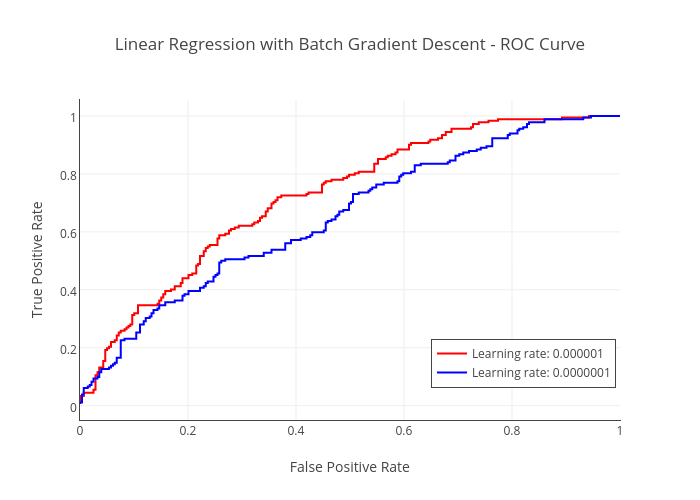
\includegraphics[width=12cm]{lin_bgd/lin_bgd_all_roc}}
\end{center}
\caption{ROC Curve of Linear Regression with BGD training with 2 different learning rates.}
\label{Fig5}
\end{figure}

\begin{figure}[!htbp]
\begin{center}
\fbox{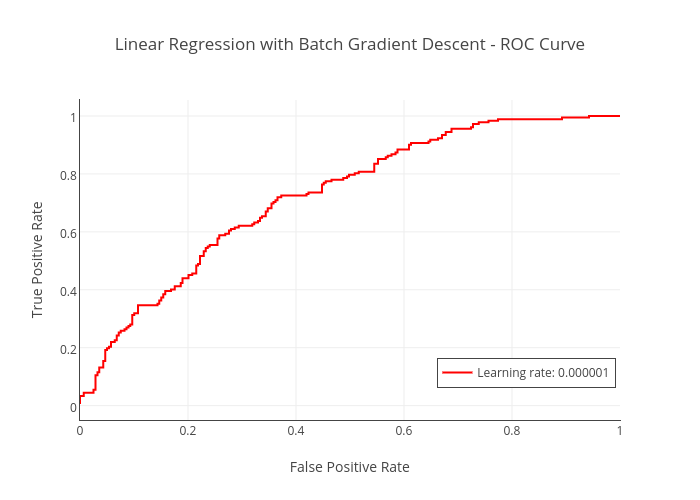
\includegraphics[width=12cm]{lin_bgd/lin_bgd_all_roc1}}
\end{center}
\caption{ROC Curve of Linear Regression with BGD training with optimal learning rate identified.}
\label{Fig6}
\end{figure}

\textbf{Area under the curve (AUC)}

Table \ref{Table4} shows the AUC (Area under the curve) of Linear Regression with BGD trained with 6 different learning rates for 50 epochs.

\begin{table}[!htbp]
\caption{AUC of Linear Regression with BGD trained with 6 different learning rates. Highest AUC shown in \textbf{bold}.}
\label{Table4}
\begin{center}
\begin{tabular}{l l l}
\multicolumn{1}{c}{\bf Epochs} &\multicolumn{1}{c}{\bf Learning Rate} &\multicolumn{1}{c}{\bf AUC}
\\ \hline \\

50 & 0.0000001 & 0.6521918941273781\\

\textbf{50} & \textbf{0.000001}  & \textbf{0.7243491275749331}\\

50 & 0.00001   & diverged\\
50 & 0.0001    & diverged\\
50 & 0.001     & diverged\\
50 & 0.01      & diverged\\
\end{tabular}
\end{center}
\end{table}

\section{Logistic Regression with Stochastic Gradient Descent \cite{ng2000cs229} \cite{roc_curve}}

\subsection{Training}

Table \ref{Table5} shows the mean squared error (MSE) on the last epoch when training Logistic Regression with SGD for 500 epochs with 4 different learning rates. It was found that it produced the lowest MSE with a learning rate of 0.1.

Figure \ref{Fig7} provides a visual representation of the performance of Logistic Regression with SGD trained with 4 different learning rates for 500 epochs.

\begin{table}[!htbp]
\caption{Logistic Regression with SGD training with 4 different learning rates. Lowest MSE on the last epoch shown in \textbf{bold}.}
\label{Table5}
\begin{center}
\begin{tabular}{l l l l l}
\multicolumn{1}{c}{\bf Epochs} &\multicolumn{1}{c}{\bf Regression}  &\multicolumn{1}{c}{\bf Gradient Descent} &\multicolumn{1}{c}{\bf Learning Rate} &\multicolumn{1}{c}{\bf Last Epoch MSE}
\\ \hline \\

500 & Logistic & Stochastic & 0.0001    & 0.1883504718522505\\
500 & Logistic & Stochastic & 0.001     & 0.15310177432780345\\
500 & Logistic & Stochastic & 0.01      & 0.11686127839170125\\

\textbf{500} & \textbf{Logistic} & \textbf{Stochastic} & \textbf{0.1} & \textbf{0.08741143950554693}\\

\end{tabular}
\end{center}
\end{table}

\begin{figure}[ht]
\begin{center}
\fbox{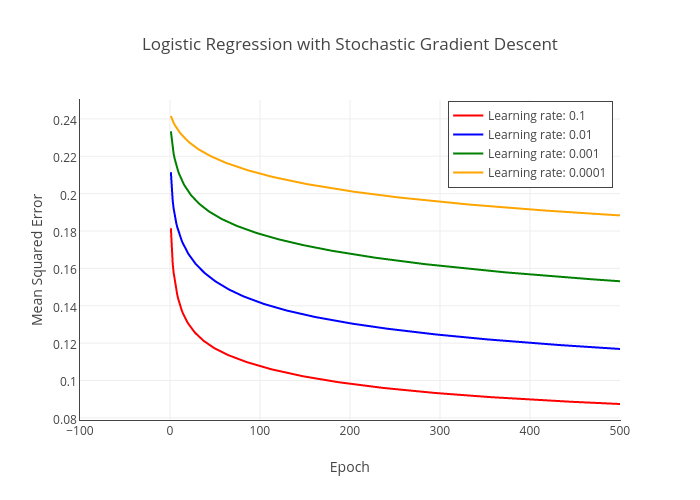
\includegraphics[width=12cm]{log_sgd/log_sgd_all}}
\end{center}
\caption{Logistic Regression with SGD training with 4 different learning rates.}
\label{Fig7}
\end{figure}

\subsection{Evaluation}

\textbf{Receiver operating characteristic (ROC) Curve}

Figure \ref{Fig8} shows the ROC curve of Logistic Regression with SGD trained with 4 different learning rates for 500 epochs.

Figure \ref{Fig9} shows the ROC curve of Logistic Regression with SGD trained with the optimal learning rate identified for 500 epochs.

\begin{figure}[!htbp]
\begin{center}
\fbox{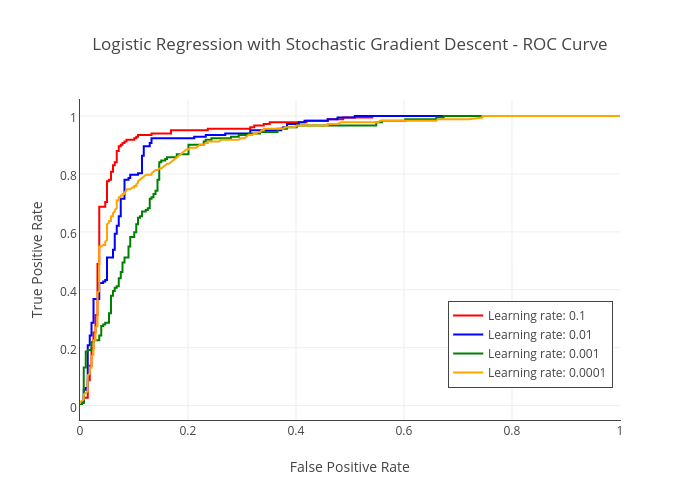
\includegraphics[width=12cm]{log_sgd/log_sgd_all_roc}}
\end{center}
\caption{ROC Curve of Logistic Regression with SGD training with 4 different learning rates.}
\label{Fig8}
\end{figure}

\begin{figure}[ht]
\begin{center}
\fbox{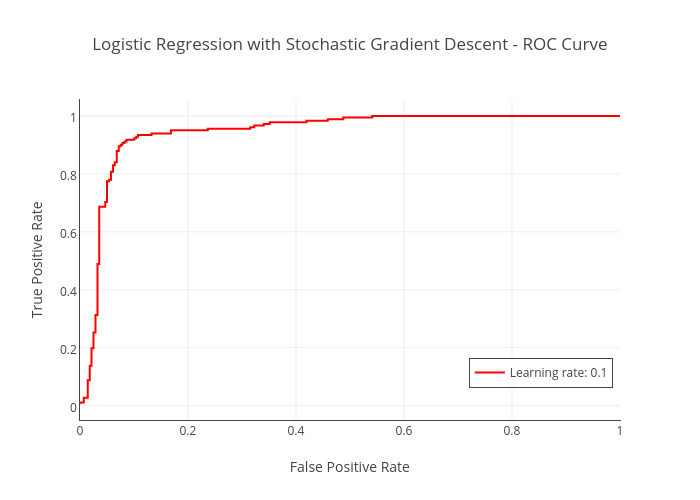
\includegraphics[width=12cm]{log_sgd/log_sgd_all_roc1}}
\end{center}
\caption{ROC Curve of Logistic Regression with SGD training with optimal learning rate identified.}
\label{Fig9}
\end{figure}

\textbf{Area under the curve (AUC)}

Table \ref{Table6} shows the AUC (Area under the curve) of Logistic Regression with SGD trained with 4 different learning rates for 500 epochs.

\begin{table}[!htbp]
\caption{AUC of Logistic Regression with SGD trained with 4 different learning rates. Highest AUC shown in \textbf{bold}.}
\label{Table6}
\begin{center}
\begin{tabular}{l l l}
\multicolumn{1}{c}{\bf Epochs} &\multicolumn{1}{c}{\bf Learning Rate} &\multicolumn{1}{c}{\bf AUC}
\\ \hline \\

500 & 0.0001 & 0.8580093741384061\\
500 & 0.001  & 0.8896963251801965\\
500 & 0.01   & 0.923431407302375\\

\textbf{500} & \textbf{0.1} & \textbf{0.9437354759935405}\\

\end{tabular}
\end{center}
\end{table}

\section{Logistic Regression with Batch Gradient Descent \cite{ng2000cs229} \cite{roc_curve}}

\subsection{Training}

Table \ref{Table7} shows the mean squared error (MSE) on the last epoch when training Logistic Regression with BGD for 50 epochs with 7 different learning rates. It was found that it produced the lowest MSE with a learning rate of 0.0001.

Figure \ref{Fig10} provides a visual representation of the performance of Logistic Regression with BGD trained with 4 different learning rates for 50 epochs.

\begin{table}[!htbp]
\caption{Logistic Regression with BGD training with 7 different learning rates. Lowest MSE on the last epoch shown in \textbf{bold}.}
\label{Table7}
\begin{center}
\begin{tabular}{l l l l l}
\multicolumn{1}{c}{\bf Epochs} &\multicolumn{1}{c}{\bf Regression}  &\multicolumn{1}{c}{\bf Gradient Descent} &\multicolumn{1}{c}{\bf Learning Rate} &\multicolumn{1}{c}{\bf Last Epoch MSE}
\\ \hline \\

50 & Logistic & Batch & 0.0000001 & 0.24895157834707887\\
50 & Logistic & Batch & 0.000001  & 0.2435508003326362\\
50 & Logistic & Batch & 0.00001   & 0.23698192269954932\\

\textbf{50} & \textbf{Logistic} & \textbf{Batch} & \textbf{0.0001} & \textbf{0.21890249704799133}\\

50 & Logistic & Batch & 0.001     & diverged\\
50 & Logistic & Batch & 0.01      & diverged\\
50 & Logistic & Batch & 0.1       & diverged\\

\end{tabular}
\end{center}
\end{table}

\begin{figure}[ht]
\begin{center}
\fbox{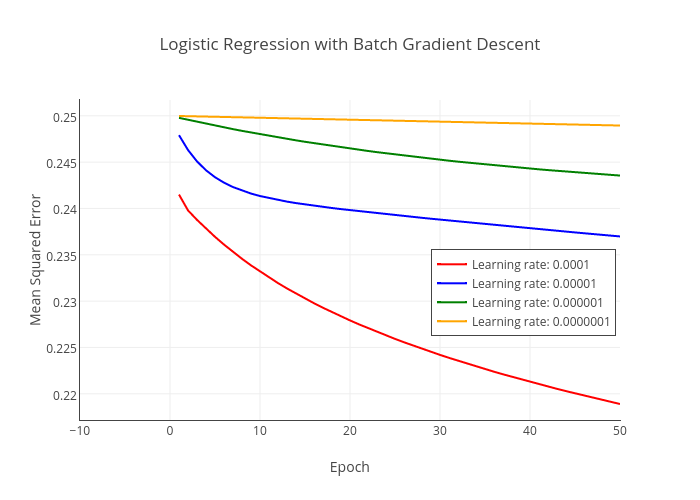
\includegraphics[width=12cm]{log_bgd/log_bgd_all}}
\end{center}
\caption{Logistic Regression with BGD training with 4 different learning rates.}
\label{Fig10}
\end{figure}

\subsection{Evaluation}

\textbf{Receiver operating characteristic (ROC) Curve}

Figure \ref{Fig11} shows the ROC curve of Logistic Regression with BGD trained with 4 different learning rates for 50 epochs.

Figure \ref{Fig12} shows the ROC curve of Logistic Regression with BGD trained with the optimal learning rate identified for 50 epochs.\newline \newline

\begin{figure}[!htbp]
\begin{center}
\fbox{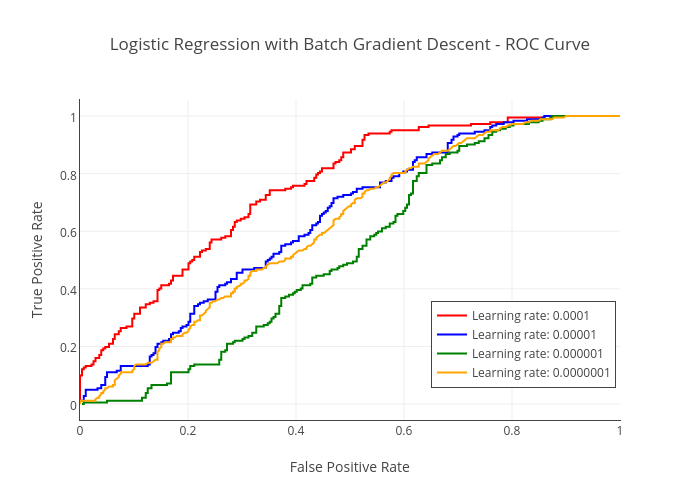
\includegraphics[width=12cm]{log_bgd/log_bgd_all_roc}}
\end{center}
\caption{ROC Curve of Logistic Regression with BGD training with 4 different learning rates.}
\label{Fig11}
\end{figure}

\begin{figure}[!htbp]
\begin{center}
\fbox{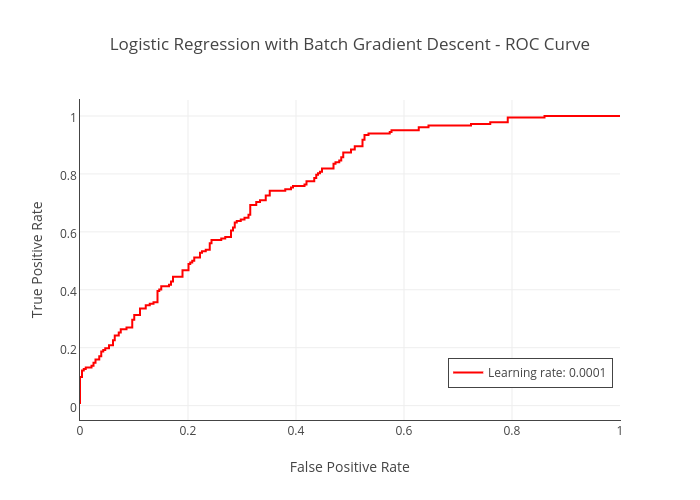
\includegraphics[width=12cm]{log_bgd/log_bgd_all_roc1}}
\end{center}
\caption{ROC Curve of Logistic Regression with BGD training with optimal learning rate identified.}
\label{Fig12}
\end{figure}

\textbf{Area under the curve (AUC)}

Table \ref{Table8} shows the AUC (Area under the curve) of Logistic Regression with BGD trained with 7 different learning rates for 50 epochs.

\begin{table}[!htbp]
\caption{AUC of Logistic Regression with BGD trained with 7 different learning rates. Highest AUC shown in \textbf{bold}.}
\label{Table8}
\begin{center}
\begin{tabular}{l l l}
\multicolumn{1}{c}{\bf Epochs} &\multicolumn{1}{c}{\bf Learning Rate} &\multicolumn{1}{c}{\bf AUC}
\\ \hline \\

50 & 0.0000001 & 0.5066761195793456\\
50 & 0.000001  & 0.528910157942416\\
50 & 0.00001   & 0.6403757532789796\\

\textbf{50} & \textbf{0.0001} & \textbf{0.7539879475363358}\\

50 & 0.001     & diverged\\
50 & 0.01      & diverged\\
50 & 0.1       & diverged\\

\end{tabular}
\end{center}
\end{table}

\section{Stochastic vs Batch Gradient Descent}

Stochastic and Batch Gradient Descent bring advantages to different scenarios mainly dependant on the size of the data. Stochastic Gradient Descent is used when data size is big. In SGD, "we repeatedly run through the training set, and each time we encounter a training example, we update the parameters according to the gradient of the error with respect to that single training example only." \cite{ng2000cs229} Batch Gradient Descent is used when data size is small. In BGD, we "scan through the entire training set before taking a single step - a costly operation if \textit{m} is large - stochastic gradient descent can start making progress right away, and continues to make progress with each example it looks at. Often, stochastic gradient descent gets \textit{\texttheta} "close" to the minimum much faster than batch gradient descent." \cite{ng2000cs229}

Because SGD only considers one example at a time, it means that it completes a single epoch faster and therefore it can also learn quicker based on the previous epoch. In comparison, BGD considers the whole data set on each epoch, which means it takes significantly longer to complete one epoch. When SGD learns, it learns from the weights of one single example. When BGD learns, it learns from a sum of weights of all examples in the data set. This leads to a slower learning process as BGD doesn't have a concrete example to learn from, instead it learns from a sum of examples.

\subsection{Stochastic vs Batch Gradient Descent for Linear Regression}

Linear Regression with Stochastic Gradient Descent was trained using 4 different learning rates for 500 epochs. The learning rates used were: 0.00001, 0.0001, 0.001 and 0.01, respectively. The Lowest MSE (0.17462479941829512) and highest AUC (0.8923549568710862) were produced using 0.001 as the learning rate. Both the MSE and AUC values produced are good.

I believe that for Linear Regression with SGD, 500 epochs is an optimal amount in order to obtain both a "good" predictor and mean squared error.

On the other hand, Linear Regression with Batch Gradient Descent was trained using 6 different learning rates for 50 epochs. The learning rates used were: 0.0000001, 0.000001, 0.00001, 0.0001, 0.001, and 0.01, respectively. The Lowest MSE (0.22658756874338298) and highest AUC (0.7243491275749331) were produced using 0.000001 as the learning rate. Both the MSE and AUC values produced are fairly average. Based on this, I believe that BGD requires to run for more than 50 epochs. However, that will also increase the time it will take to run, considering that BGD is an already slower process than SGD.

In comparison, SGD has an undeniably faster and better learning process in comparison to BGD as the difference in MSE and AUC between the two is 0.051962769 and 0.168005829, respectively. However, I believe that if run for enough epochs, BGD for Linear Regression could get close to SGD's performance.

As a result of this comparison, I attempted to run Linear Regression with Batch Gradient Descent for 2000 epochs. Tables \ref{Table9} and \ref{Table10} provide a numerical representation of this attempt, while Figures \ref{Fig13} and \ref{Fig14} provide a visual representation of it.

\begin{table}[!htbp]
\caption{Linear Regression with BGD trained with 0.000001 as the learning rate for 2000 epochs.}
\label{Table9}
\begin{center}
\begin{tabular}{l l l l l}
\multicolumn{1}{c}{\bf Epochs} &\multicolumn{1}{c}{\bf Regression}  &\multicolumn{1}{c}{\bf Gradient Descent} &\multicolumn{1}{c}{\bf Learning Rate} &\multicolumn{1}{c}{\bf Last Epoch MSE}
\\ \hline \\

2000 & Linear & Batch & 0.000001 & 0.19789523905781295\\

\end{tabular}
\end{center}
\end{table}

\begin{table}[!htbp]
\caption{AUC of Linear Regression with BGD trained with 0.000001 as the learning rate for 2000 epochs.}
\label{Table10}
\begin{center}
\begin{tabular}{l l l}
\multicolumn{1}{c}{\bf Epochs} &\multicolumn{1}{c}{\bf Learning Rate} &\multicolumn{1}{c}{\bf AUC}
\\ \hline \\

2000 & 0.000001 & 0.8280751506557958\\

\end{tabular}
\end{center}
\end{table}

\begin{figure}[!htbp]
\begin{center}
\fbox{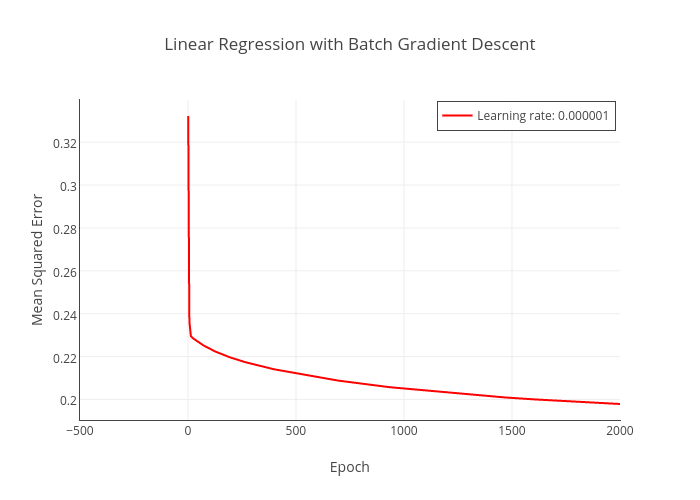
\includegraphics[width=12cm]{lin_bgd/lin_bgd_0_000001_2000}}
\end{center}
\caption{Linear Regression with BGD trained with 0.000001 as the learning rate for 2000 epochs.}
\label{Fig13}
\end{figure}

\begin{figure}[!htbp]
\begin{center}
\fbox{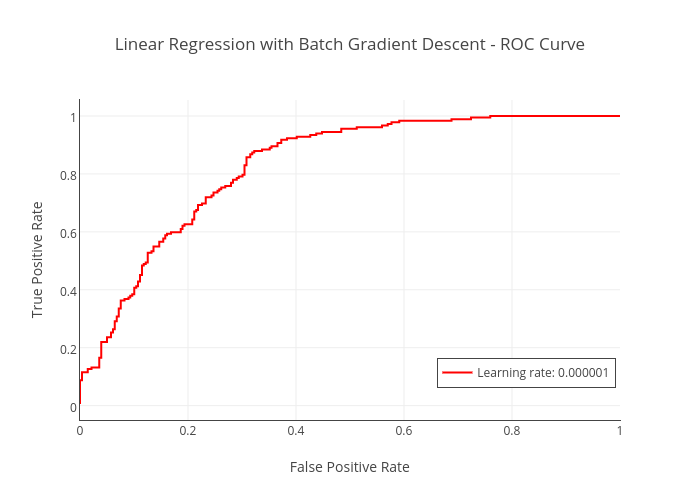
\includegraphics[width=12cm]{lin_bgd/lin_bgd_0_000001_2000_roc}}
\end{center}
\caption{ROC Curve of Linear Regression with BGD trained with 0.000001 as the learning rate for 2000 epochs.}
\label{Fig14}
\end{figure}

\subsection{Stochastic vs Batch Gradient Descent for Logistic Regression}

Logistic Regression with Stochastic Gradient Descent was trained using 4 different learning rates for 500 epochs. The learning rates used were: 0.0001, 0.001, 0.01 and 0.1, respectively. Lowest MSE (0.08741143950554693) and highest AUC (0.9437354759935405) were produced using 0.1 as the learning rate. Both the MSE and AUC values produced are good.

I believe that for Logistic Regression with SGD, 500 epochs is an optimal amount in order to obtain both a "good" predictor and mean squared error.

On the other hand, Logistic Regression with Batch Gradient Descent was trained using 7 different learning rates for 50 epochs. The learning rates used were: 0.0000001, 0.000001, 0.00001, 0.0001, 0.001, 0.01 and 0.1, respectively. Lowest MSE (0.21890249704799133) and highest AUC (0.7539879475363358) were produced using 0.0001 as the learning rate. Both the MSE and AUC values produced are fairly average. Based on this, I believe that BGD requires to run for more than 50 epochs. However, that will also increase the time it will take to run, considering that BGD is an already slower process than SGD.

In comparison, SGD has an undeniably faster and better learning process as the difference in MSE and AUC between the two is 0.131491058 and 0.189747528, respectively. However, I believe that if run for enough epochs, BGD for Logistic Regression could get close to SGD's performance.

As a result of this comparison, I attempted to run Logistic Regression with Batch Gradient Descent for 2000 epochs. Tables \ref{Table11} and \ref{Table12} provide a numerical representation of this attempt, while Figures \ref{Fig15} and \ref{Fig16} (next page provide a visual representation of it.

\begin{table}[!htbp]
\caption{Logistic Regression with BGD trained with 0.0001 as the learning rate for 2000 epochs.}
\label{Table11}
\begin{center}
\begin{tabular}{l l l l l}
\multicolumn{1}{c}{\bf Epochs} &\multicolumn{1}{c}{\bf Regression}  &\multicolumn{1}{c}{\bf Gradient Descent} &\multicolumn{1}{c}{\bf Learning Rate} &\multicolumn{1}{c}{\bf Last Epoch MSE}
\\ \hline \\

2000 & Logistic & Batch & 0.0001 & 0.16774604152828332\\

\end{tabular}
\end{center}
\end{table}

\begin{table}[!htbp]
\caption{AUC of Logistic Regression with BGD trained with 0.0001 as the learning rate for 2000 epochs.}
\label{Table12}
\begin{center}
\begin{tabular}{l l l}
\multicolumn{1}{c}{\bf Epochs} &\multicolumn{1}{c}{\bf Learning Rate} &\multicolumn{1}{c}{\bf AUC}
\\ \hline \\

2000 & 0.0001 & 0.8764425538619093\\

\end{tabular}
\end{center}
\end{table}

\clearpage

\begin{figure}[!htbp]
\begin{center}
\fbox{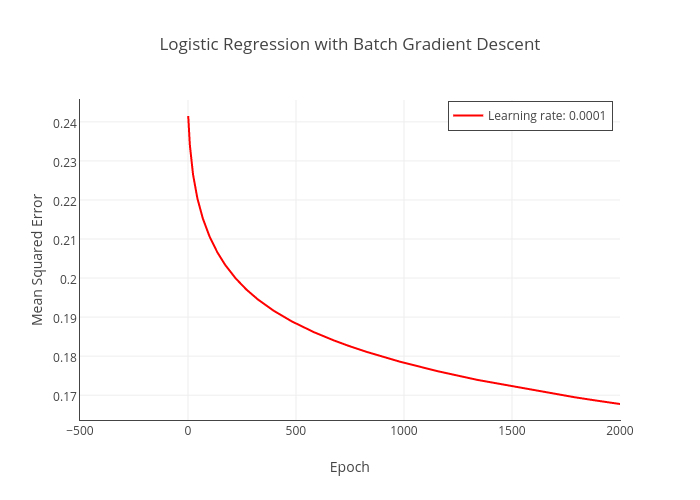
\includegraphics[width=12cm]{log_bgd/log_bgd_0_0001_2000}}
\end{center}
\caption{Logistic Regression with BGD trained with 0.0001 as the learning rate for 2000 epochs.}
\label{Fig15}
\end{figure}

\begin{figure}[!htbp]
\begin{center}
\fbox{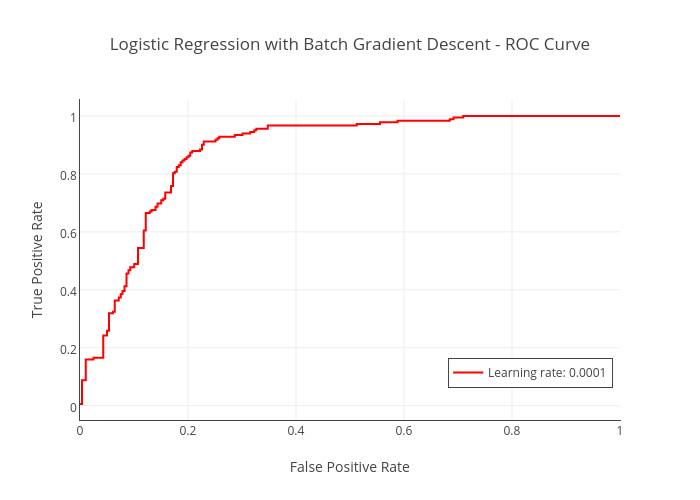
\includegraphics[width=12cm]{log_bgd/log_bgd_0_0001_2000_roc}}
\end{center}
\caption{ROC Curve of Logistic Regression with BGD trained with 0.0001 as the learning rate for 2000 epochs.}
\label{Fig16}
\end{figure}

\clearpage

\nocite{python_list_comprehensions, python_zip, python_sum, plotly}
\printbibliography
\end{document}